\section{Date: 2026-07-21}
\noindent \textbf{Series ID: TREAS1T5} 

\noindent This series is titled Assets: Securities Held Outright: U.S. Treasury Securities: Maturing in over 1 Year to 5 Years: Wednesday Level and has a frequency of Weekly, As of Wednesday. The units are Millions of U.S. Dollars and the seasonal adjustment is Not Seasonally Adjusted.The observation start date is 2002-12-18 and the observation end date is 2026-07-15.The popularity of this series is 21. \\ 

\noindent \textbf{Series ID: CUURD300SAS} 

\noindent This series is titled Consumer Price Index for All Urban Consumers: Services in South - Size Class D (DISCONTINUED) and has a frequency of Monthly. The units are Index 1982-1984=100 and the seasonal adjustment is Not Seasonally Adjusted.The observation start date is 1977-12-01 and the observation end date is 2017-12-01.The popularity of this series is 1. \\ 

\subsection{Raw Regression}
\noindent Regresses the two series against each other directly. A significant result here can come just as easily from both series sharing a long-run trend as from any real relationship.

\begin{center}
\begin{tabular}{lclc}
\toprule
\textbf{Dep. Variable:}        & value\_fred\_CUURD300SAS & \textbf{  R-squared:         } &     0.774   \\
\textbf{Model:}                &           OLS            & \textbf{  Adj. R-squared:    } &     0.765   \\
\textbf{Method:}               &      Least Squares       & \textbf{  F-statistic:       } &     82.38   \\
\textbf{Date:}                 &     Tue, 21 Jul 2026     & \textbf{  Prob (F-statistic):} &  3.15e-09   \\
\textbf{Time:}                 &         13:11:10         & \textbf{  Log-Likelihood:    } &   -104.86   \\
\textbf{No. Observations:}     &              26          & \textbf{  AIC:               } &     213.7   \\
\textbf{Df Residuals:}         &              24          & \textbf{  BIC:               } &     216.2   \\
\textbf{Df Model:}             &               1          & \textbf{                     } &             \\
\textbf{Covariance Type:}      &        nonrobust         & \textbf{                     } &             \\
\bottomrule
\end{tabular}
\begin{tabular}{lcccccc}
                               & \textbf{coef} & \textbf{std err} & \textbf{t} & \textbf{P$> |$t$|$} & \textbf{[0.025} & \textbf{0.975]}  \\
\midrule
\textbf{const}                 &     214.5017  &        4.768     &    44.985  &         0.000        &      204.660    &      224.343     \\
\textbf{value\_fred\_TREAS1T5} &    6.405e-05  &     7.06e-06     &     9.076  &         0.000        &     4.95e-05    &     7.86e-05     \\
\bottomrule
\end{tabular}
\begin{tabular}{lclc}
\textbf{Omnibus:}       &  1.003 & \textbf{  Durbin-Watson:     } &    0.294  \\
\textbf{Prob(Omnibus):} &  0.606 & \textbf{  Jarque-Bera (JB):  } &    0.795  \\
\textbf{Skew:}          & -0.004 & \textbf{  Prob(JB):          } &    0.672  \\
\textbf{Kurtosis:}      &  2.143 & \textbf{  Cond. No.          } & 1.16e+06  \\
\bottomrule
\end{tabular}
%\caption{OLS Regression Results}
\end{center}

Notes: \newline
 [1] Standard Errors assume that the covariance matrix of the errors is correctly specified. \newline
 [2] The condition number is large, 1.16e+06. This might indicate that there are \newline
 strong multicollinearity or other numerical problems.

\begin{figure}
\centering
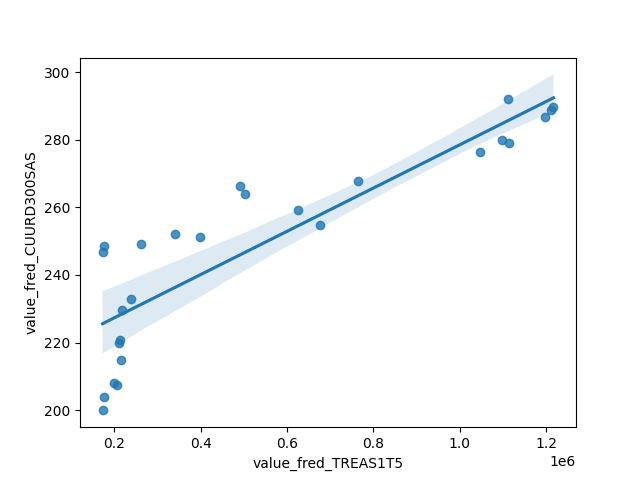
\includegraphics[scale = 0.9]{plots/plot_2026-07-21.png}
\caption{Raw Regression Plot for 2026-07-21}
\end{figure}
\newpage
\subsection{Detrended Regression}
\noindent Regresses the residuals of each series after removing its own linear time trend, so a shared trend can no longer drive the result on its own. A relationship that stays significant here is better evidence of a genuine link between the two series.

\begin{center}
\begin{tabular}{lclc}
\toprule
\textbf{Dep. Variable:}                   & value\_fred\_CUURD300SAS\_detrended & \textbf{  R-squared:         } &     0.365   \\
\textbf{Model:}                           &                 OLS                 & \textbf{  Adj. R-squared:    } &     0.339   \\
\textbf{Method:}                          &            Least Squares            & \textbf{  F-statistic:       } &     13.82   \\
\textbf{Date:}                            &           Tue, 21 Jul 2026          & \textbf{  Prob (F-statistic):} &  0.00107    \\
\textbf{Time:}                            &               13:11:11              & \textbf{  Log-Likelihood:    } &   -63.094   \\
\textbf{No. Observations:}                &                    26               & \textbf{  AIC:               } &     130.2   \\
\textbf{Df Residuals:}                    &                    24               & \textbf{  BIC:               } &     132.7   \\
\textbf{Df Model:}                        &                     1               & \textbf{                     } &             \\
\textbf{Covariance Type:}                 &              nonrobust              & \textbf{                     } &             \\
\bottomrule
\end{tabular}
\begin{tabular}{lcccccc}
                                          & \textbf{coef} & \textbf{std err} & \textbf{t} & \textbf{P$> |$t$|$} & \textbf{[0.025} & \textbf{0.975]}  \\
\midrule
\textbf{const}                            &    4.318e-12  &        0.559     &  7.72e-12  &         1.000        &       -1.154    &        1.154     \\
\textbf{value\_fred\_TREAS1T5\_detrended} &   -1.309e-05  &     3.52e-06     &    -3.718  &         0.001        &    -2.04e-05    &    -5.83e-06     \\
\bottomrule
\end{tabular}
\begin{tabular}{lclc}
\textbf{Omnibus:}       &  0.194 & \textbf{  Durbin-Watson:     } &    1.006  \\
\textbf{Prob(Omnibus):} &  0.907 & \textbf{  Jarque-Bera (JB):  } &    0.403  \\
\textbf{Skew:}          &  0.028 & \textbf{  Prob(JB):          } &    0.818  \\
\textbf{Kurtosis:}      &  2.393 & \textbf{  Cond. No.          } & 1.59e+05  \\
\bottomrule
\end{tabular}
%\caption{OLS Regression Results}
\end{center}

Notes: \newline
 [1] Standard Errors assume that the covariance matrix of the errors is correctly specified. \newline
 [2] The condition number is large, 1.59e+05. This might indicate that there are \newline
 strong multicollinearity or other numerical problems.

\begin{figure}
\centering
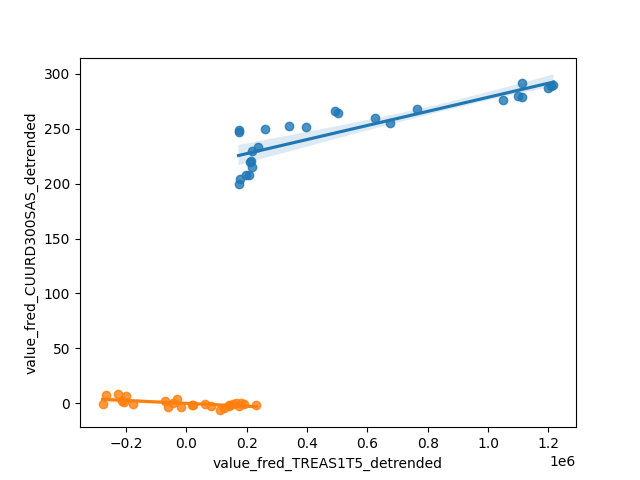
\includegraphics[scale = 0.9]{plots/plot_2026-07-21_detrended.png}
\caption{Detrended Regression Plot for 2026-07-21}
\end{figure}
\newpage
